\documentclass[sigconf,review,anonymous]{acmart}

% For an ACM journal-style submission, consider replacing the documentclass with:
% \documentclass[acmsmall,review,anonymous]{acmart}
% For a preprint, remove review/anonymous and set printacmref=false below.

\AtBeginDocument{%
  \providecommand\BibTeX{{%
    Bib\TeX}}}

\setcopyright{none}
\settopmatter{printacmref=false, printccs=false, printfolios=true}
\renewcommand\footnotetextcopyrightpermission[1]{}

\usepackage{booktabs}
\usepackage{array}
\usepackage{enumitem}
\usepackage{xspace}
\usepackage{balance}
\usepackage{graphicx}
\usepackage{multirow}
\usepackage{pifont}
\usepackage{amsmath}
\usepackage{amsfonts}

\newcommand{\system}{SEPA-Eval\xspace}
\newcommand{\todo}[1]{\textcolor{red}{[TODO: #1]}}

\begin{document}

\title{Self-Evolving Agents for Physical AI Evaluation}
\subtitle{From Static Benchmarks to Living Evaluation Systems for World Models and Robotic Foundation Models}

\author{Author One}
\affiliation{%
  \institution{Institution}
  \city{City}
  \country{Country}}
\email{author@example.com}

\author{Author Two}
\affiliation{%
  \institution{Institution}
  \city{City}
  \country{Country}}
\email{author2@example.com}

\begin{abstract}
Physical AI systems increasingly combine world models, simulation, and vision-language-action policies to perceive, predict, and act in the physical world. However, evaluation remains largely static, fragmented, and weakly calibrated to real-world deployment. Fixed benchmarks can saturate, miss emerging failure modes, and fail silently as model capabilities shift. We propose \system, a self-evolving evaluation architecture for Physical AI. \system continuously generates new embodied tasks, evaluates world models and robot policies jointly, mines failures and sim-real disagreements, calibrates critic ensembles with real-world outcomes, and updates benchmark distributions over time. The architecture centers on an evaluation memory that stores tasks, rollouts, predictions, plans, critic judgments, failures, explanations, metrics, and human feedback. We argue that the central metric for Physical AI evaluation should be predictive validity: whether evaluation results forecast real-world robot behavior and reveal the next frontier of failures. This white paper outlines the architecture, metric taxonomy, research agenda, and implementation roadmap for living evaluation infrastructure for embodied AI.
\end{abstract}

\maketitle

\section{Introduction}

Physical AI is entering a new phase. World models can generate plausible futures, simulators can produce large-scale synthetic robot experience, and vision-language-action (VLA) models are becoming general-purpose robotic policies. Yet evaluation remains largely static: fixed task lists, fixed simulators, fixed metrics, and fixed success definitions. This creates a dangerous mismatch. A model can appear to improve on a benchmark while the benchmark itself becomes less informative, less discriminative, or less predictive of deployment behavior.

This white paper proposes a new evaluation paradigm: \emph{self-evolving agents for Physical AI evaluation}. Instead of treating evaluation as a one-time benchmark, we propose an agentic system that observes model behavior, mines failures, generates new tests, validates them in simulation and the real world, updates the evaluation suite, and tracks when existing evals become obsolete. This framing is motivated by recent arguments that evaluation protocols themselves break as model capabilities shift~\cite{wang2025evalsbreak}, and extends that argument to embodied systems where failures can arise from contact dynamics, sensing, language grounding, planning, control, safety, and sim-to-real mismatch.

We focus on two coupled model families. The first is \emph{world models}: video/action-conditioned predictors, neural simulators, object-centric dynamics models, and foundation world models. The second is \emph{robotics models}: VLA policies, diffusion or flow-based policies, hierarchical controllers, and multi-embodiment robot foundation models. Our core claim is that these systems should not be evaluated separately. A world model is useful only if it preserves the physical and causal structure needed for embodied action. A robot policy is trustworthy only if it remains robust under meaningful physical variation.

\begin{quote}
\emph{Physical AI should not be evaluated only by asking whether a robot succeeds on today's tasks. It should be evaluated by asking whether the evaluation system can continuously discover tomorrow's failures.}
\end{quote}

\section{Why Static Physical AI Evaluation Fails}

Evaluation is often treated as a fixed measurement problem: choose a benchmark, define metrics, run models, and compare scores. This paradigm is insufficient for Physical AI. Embodied agents interact with the world through perception, language, planning, control, and contact-rich dynamics. Their failures are rarely one-dimensional. A robot may understand the instruction but misjudge an affordance; predict free-space motion correctly but fail at contact; succeed under ideal lighting but fail under reflection, transparency, clutter, or a slight camera shift; or pass a simulator benchmark by exploiting simulator artifacts.

Static benchmarks fail in at least three ways.

\textbf{Saturation.} Once models exceed the difficulty level of a benchmark, the benchmark no longer separates frontier systems.

\textbf{Misalignment.} A benchmark may reward shallow success while missing what matters for deployment: safety, recovery, robustness, calibration, and predictive validity.

\textbf{Silent failure.} Scores may continue to look meaningful even when they no longer predict real-world outcomes.

These failure modes are especially dangerous in robotics because embodied failures can be costly, unsafe, and difficult to reproduce. The next generation of evaluation should therefore be adaptive: it should observe failures, generate tests around them, validate those tests, and update the benchmark distribution.

\section{Related Work and Resource Landscape}

\subsection{VLA and robot foundation models}

VLA models map visual observations and language instructions into robot actions. RT-2 introduced a VLA recipe that incorporates web-scale vision-language pretraining directly into robotic control~\cite{brohan2023rt2}. OpenVLA provides a widely used open-source 7B-parameter VLA trained on large-scale robot demonstrations~\cite{kim2024openvla}. $\pi_0$ proposes a vision-language-action flow model for general robot control, trained across multiple dexterous robot platforms~\cite{black2024pi0}. Industrial systems such as Isaac GR00T N1 further signal movement toward large robot foundation models for humanoids~\cite{nvidia2025groot}.

These advances intensify the need for stronger evaluation. A fixed set of tabletop manipulation tasks cannot fully test physical reasoning, long-horizon execution, cross-embodiment transfer, safety, or robustness under environmental variation.

\subsection{World-model evaluation}

World models can serve as synthetic data engines, policy evaluators, action planners, safety forecasters, counterfactual generators, and learned simulators. WorldArena emphasizes that embodied world models should be evaluated not only by perceptual quality but also by functional utility, including use as data engines, policy evaluators, and planners~\cite{worldarena2026}. WorldModelBench highlights world-model-specific violations such as instruction-following and physics-adherence failures~\cite{worldmodelbench2025}. Physion and Physion-Eval focus on physical realism and human physical reasoning in generated videos~\cite{physionatlas2025,physioneval2026}. Morpheus evaluates physical conservation properties in generated video~\cite{morpheus2025}.

For robotics, the key point is that visual realism is not enough. RoboWM-Bench argues that visually plausible generated behavior may still fail when converted into executable robot actions, and proposes embodiment-grounded evaluation of world models in manipulation~\cite{jiang2026robowm}. WorldEval studies whether world models can serve as scalable proxies for real-world robot-policy evaluation~\cite{li2025worldeval}, while dWorldEval extends this direction with discrete diffusion world models for scalable policy evaluation~\cite{dworldeval2026}.

\subsection{Embodied simulation and task benchmarks}

Large-scale simulation benchmarks provide the substrate for evolving evaluation distributions. RoboCasa provides realistic household environments and tasks for generalist robot learning~\cite{nasiriany2024robocasa}. RoboCasa365 expands toward large-scale household mobile manipulation, multi-task learning, foundation model training, and lifelong learning~\cite{robocasa3652026}. BEHAVIOR-1K introduces 1,000 human-centered everyday activities across realistic scenes with rich physical and semantic object properties~\cite{li2024behavior1k}. Such benchmarks are essential, but we argue that they should become sources of evolving test distributions rather than fixed leaderboards.

\section{Architecture Overview}

Figure~\ref{fig:architecture} summarizes the proposed architecture. The system contains seven major components: subject models, task and scenario evolution, world-model evaluation, VLA/robot evaluation, critic ensembles, sim-real calibration, and evaluation memory.

\begin{figure*}[t]
  \centering
  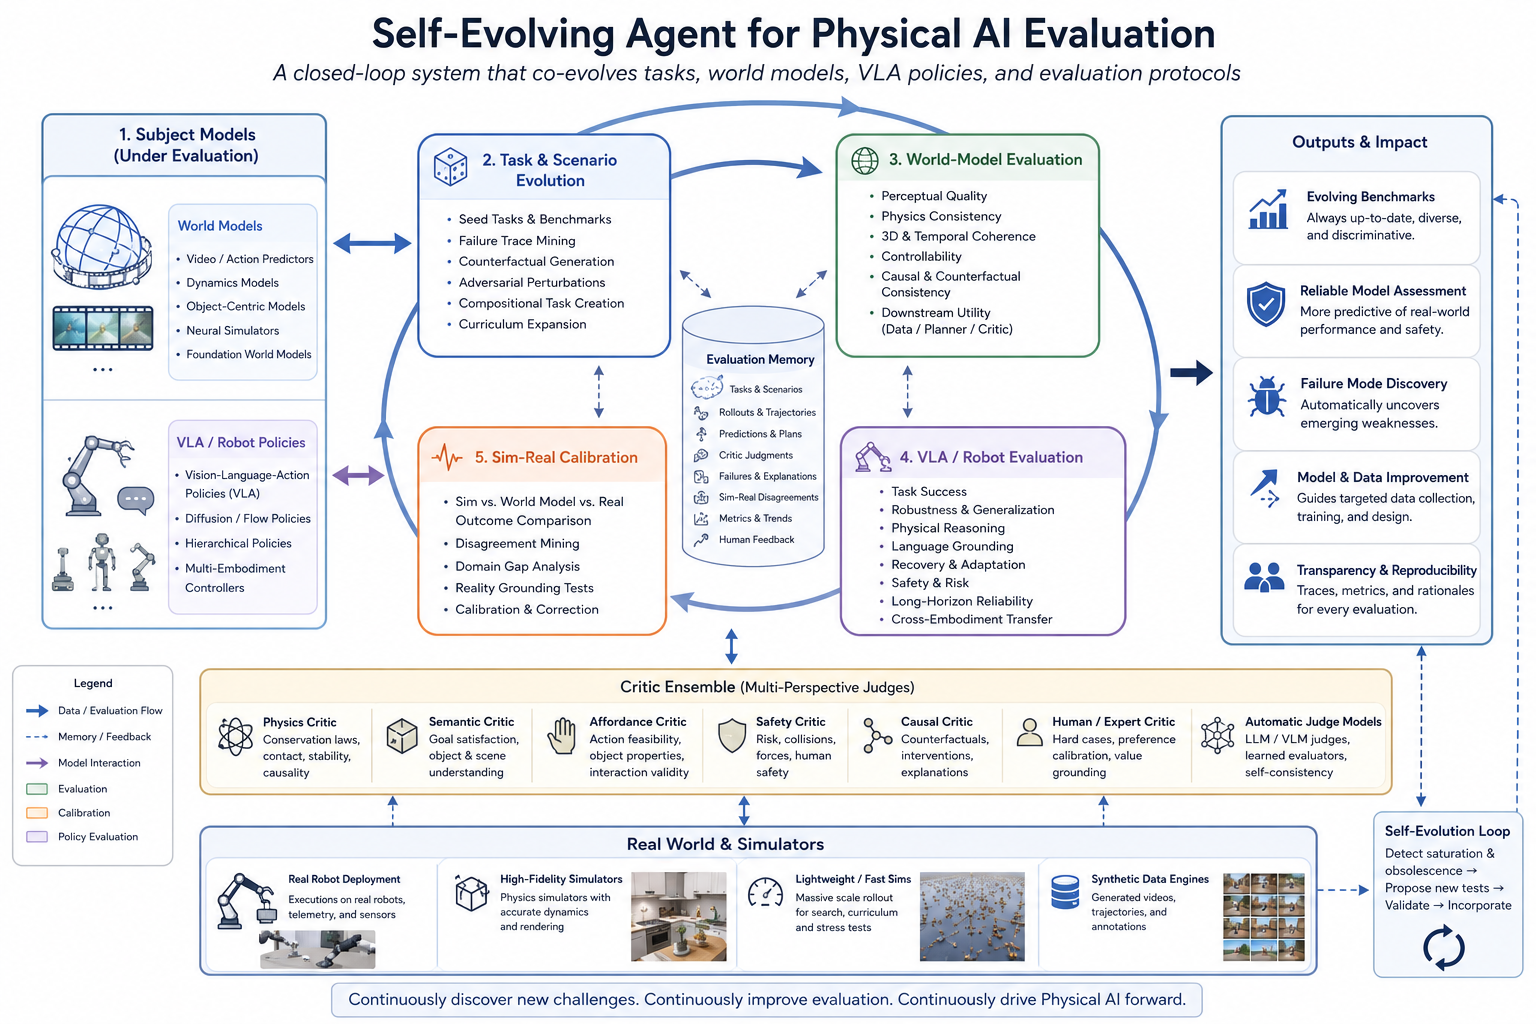
\includegraphics[width=0.98\textwidth]{figures/system_architecture.png}
  \caption{Self-evolving agent for Physical AI evaluation. The architecture treats evaluation as a closed-loop system that co-evolves tasks, world models, robot policies, critic ensembles, simulators, real-world rollouts, and evaluation protocols. The central evaluation memory stores tasks, rollouts, predictions, plans, critic judgments, failures, metrics, and human feedback.}
  \label{fig:architecture}
\end{figure*}

The design principle is that evaluation outputs are not the end of the process. They feed back into the next generation of tasks, critics, metrics, and model-improvement signals. The evaluator is itself an agent: it observes behavior, forms hypotheses about weaknesses, designs experiments, runs them across world models and robots, and updates the evaluation suite.

\section{Subject Models Under Evaluation}

\subsection{World models}

World models include video prediction models, action-conditioned video models, object-centric dynamics models, neural simulators, learned physical predictors, foundation world models, and hybrid simulator-neural models. They should be evaluated both as generative models and as functional components in the robotics stack.

A world model used for robotics should satisfy five forms of validity:

\begin{enumerate}[leftmargin=*]
  \item \textbf{Perceptual validity}: does the generated future look realistic?
  \item \textbf{Physical validity}: does it obey relevant physical constraints?
  \item \textbf{Causal validity}: does it correctly predict effects of actions and interventions?
  \item \textbf{Behavioral validity}: does it predict robot policy success or failure?
  \item \textbf{Deployment validity}: does it correlate with real-world robot outcomes?
\end{enumerate}

\subsection{VLA and robot policies}

Robot policies include VLA policies, diffusion policies, flow-matching action policies, hierarchical planners and controllers, multi-embodiment policies, mobile manipulation policies, and humanoid policies. The evaluation system should treat policies not only as black-box success-rate generators, but as behavioral systems with traces, decisions, recoveries, and failure modes.

\section{Task and Scenario Evolution}

The task evolution module generates new evaluation cases from multiple sources.

\subsection{Seed tasks and benchmarks}

The system begins from existing benchmarks, task suites, and real-world deployment scenarios. These provide initial coverage but should not be treated as sufficient.

\subsection{Failure trace mining}

Every failed rollout is a source of new tests. The agent extracts the attempted goal, physical context, action preceding failure, whether the model perceived the failure, whether recovery was attempted, and whether the cause was perception, planning, control, physics, language grounding, or embodiment mismatch.

\subsection{Counterfactual generation}

The agent generates counterfactual variants: same task with different object pose; same instruction with distractors; same scene with altered lighting; same manipulation with changed mass or friction; same goal with a different tool; same success case with added human interruption.

\subsection{Adversarial physical perturbation}

The system searches for minimal physical changes that cause failure, such as small camera shifts, occlusion, reflective surfaces, transparent objects, unstable stacks, slippery contact, deformable objects, cables, clutter, and ambiguous language.

\subsection{Curriculum expansion}

When models begin to solve a task family, the system expands difficulty: longer horizon, more objects, more distractors, less observability, stricter safety constraints, more ambiguous instructions, higher physical precision, and more recovery requirements.

\section{World-Model Evaluation}

World-model evaluation should combine perceptual, physical, causal, and functional metrics.

\subsection{Perceptual and temporal quality}

Perceptual metrics ask whether the generated future looks plausible. They include visual fidelity, temporal coherence, frame consistency, object appearance stability, scene consistency, and camera motion realism. These metrics are useful but insufficient.

\subsection{Physical consistency}

Physical consistency tests whether the model obeys action-relevant constraints: object permanence, collision consistency, contact stability, gravity and support, rigid-body motion, deformable-object behavior, liquid behavior, friction and slip, containment, causality, and reversibility.

\subsection{3D and spatial consistency}

Robotics requires more than 2D video realism. The system should test depth consistency, object-pose stability, view consistency, occlusion handling, spatial relations, affordance geometry, and reachability.

\subsection{Controllability}

A world model used for robotics must follow action conditions. It should not merely generate plausible futures; it should generate futures that reflect commanded actions. Useful tests include same-scene/different-action comparisons, action ablations, counterfactual action comparisons, trajectory-conditioned generation, and success/failure prediction under alternative plans.

\subsection{Downstream robot utility}

The most important question is whether the world model helps robotics. The system should evaluate whether the world model can generate synthetic data that improves policies, rank policies similarly to real-world evaluation, support action planning, detect unsafe futures, identify failure causes, improve recovery policies, and reduce real-world trial cost.

\section{VLA and Robot Policy Evaluation}

Robot policy evaluation should go beyond task success.

\subsection{Task success}

Success should be measured at multiple levels: binary completion, partial progress, time to completion, number of interventions, action efficiency, energy or force efficiency, collateral damage, and final-state quality.

\subsection{Robustness and generalization}

The system should test whether success survives distribution shift: object pose changes, object shape changes, material changes, lighting changes, camera shifts, clutter, distractors, language paraphrases, unseen object categories, unseen scenes, and different embodiments.

\subsection{Physical reasoning}

The system should evaluate whether the robot handles support, stability, containment, force, friction, deformation, tool use, collision, reachability, occlusion, and irreversibility.

\subsection{Language-grounded action}

The policy should bind language to objects, attributes, relations, constraints, subgoals, safety requirements, temporal order, and exception conditions.

\subsection{Recovery and adaptation}

Deployed robots must handle failure. The evaluation should measure failure detection, self-correction, retry strategy, replanning, asking for help, safe fallback, and graceful degradation.

\subsection{Safety and risk}

Safety should be a first-class metric. Tests should include collision risk, excessive force, dropping or spilling, damaging fragile objects, unsafe proximity to humans, sharp or hot objects, irreversible actions, unsafe exploration, and out-of-distribution uncertainty.

\section{Critic Ensemble}

No single metric can judge Physical AI. \system uses a critic ensemble:

\begin{itemize}[leftmargin=*]
  \item \textbf{Physics critic}: gravity, support, contact, collision, conservation, deformation, and causal continuity.
  \item \textbf{Semantic critic}: task completion, object correctness, constraint satisfaction, and instruction following.
  \item \textbf{Affordance critic}: graspability, tool appropriateness, reachability, and manipulation feasibility.
  \item \textbf{Safety critic}: collisions, spills, breakage, human proximity, unsafe forces, and irreversible operations.
  \item \textbf{Causal critic}: interventions, failure causes, and counterfactual explanations.
  \item \textbf{Human/expert critic}: calibration, edge cases, ambiguous tasks, and high-stakes judgments.
  \item \textbf{Automatic judge models}: scalable LLM/VLM-based evaluation calibrated against humans, physics engines, and real outcomes.
\end{itemize}

The critic ensemble should produce not only scores, but also explanations and uncertainty estimates.

\section{Sim-Real Calibration}

The sim-real calibration loop compares outcomes across world-model predictions, simulator rollouts, and real robot executions. The most valuable cases are disagreements:

\begin{itemize}[leftmargin=*]
  \item world model predicts success, simulator predicts success, real robot fails;
  \item simulator predicts failure, real robot succeeds;
  \item world model predicts safety, real rollout is unsafe;
  \item policy succeeds in one embodiment but fails in another;
  \item synthetic data improves simulator success but hurts real-world performance.
\end{itemize}

These disagreements define the frontier of evaluation uncertainty. The agent should mine them and turn them into new tests. Calibration should measure rank correlation between simulated and real policy performance, task-level success correlation, failure-mode overlap, trajectory similarity, contact-event similarity, distribution-shift sensitivity, confidence calibration, and real-world predictive validity.

\section{Evaluation Memory}

Evaluation memory stores task definitions, scene configurations, object metadata, robot embodiments, policy versions, world-model versions, simulator settings, rollouts, videos, trajectories, actions, rewards, success labels, critic judgments, human feedback, failure explanations, sim-real disagreements, benchmark saturation history, and metric drift.

This memory lets the system answer: which tasks are saturated; which tasks still discriminate frontier models; which failures recur across model families; which simulator results correlate with reality; which world-model metrics predict downstream utility; and which generated tests should be promoted into the official benchmark.

\section{The Self-Evolution Loop}

\system iterates through seven steps.

\begin{enumerate}[leftmargin=*]
  \item \textbf{Evaluate}: run world models and robot policies on the current task distribution.
  \item \textbf{Diagnose}: cluster failures into perception, language, physics, contact, control, planning, recovery, safety, sim-real, world-model, or judge failures.
  \item \textbf{Generate}: create task candidates by perturbing scenes, composing subgoals, increasing horizon, varying physics parameters, and replaying failures.
  \item \textbf{Validate}: check physical validity, reproducibility, solvability, diversity, non-redundancy, discriminative power, real-world relevance, and safety relevance.
  \item \textbf{Promote}: add high-value tests to the benchmark distribution.
  \item \textbf{Monitor obsolescence}: track saturation, discriminative power, predictive validity, and metric gaming.
  \item \textbf{Report}: summarize capability frontiers, recurring failures, robustness cliffs, sim-real gaps, safety risks, and recommended next tests.
\end{enumerate}

\section{Metrics}

Table~\ref{tab:metrics} summarizes metric families for world models, robot policies, and the self-evolving evaluator itself.

\begin{table*}[t]
\centering
\caption{Metric families for self-evolving Physical AI evaluation.}
\label{tab:metrics}
\begin{tabular}{p{0.22\textwidth}p{0.32\textwidth}p{0.38\textwidth}}
\toprule
\textbf{Target} & \textbf{Metric family} & \textbf{Example questions} \\
\midrule
\multirow{6}{*}{World model}
& Visual and temporal realism & Does the generated future look plausible and remain coherent? \\
& Physical consistency & Are contact, gravity, support, deformation, and friction plausible? \\
& 3D/spatial consistency & Are pose, depth, occlusion, and affordance geometry stable? \\
& Action controllability & Does the future change correctly under different actions? \\
& Causal consistency & Do interventions lead to expected consequences? \\
& Downstream utility & Does the model improve synthetic data, planning, policy ranking, or safety forecasting? \\
\midrule
\multirow{6}{*}{Robot policy}
& Task success & Does the robot complete the task under constraints? \\
& Robustness & Does success survive perturbations? \\
& Generalization & Does it transfer across objects, scenes, and embodiments? \\
& Physical reasoning & Does it handle support, contact, friction, stability, and tool use? \\
& Recovery and safety & Can it detect failure, replan, and avoid unsafe outcomes? \\
& Calibration & Does confidence reflect actual success probability? \\
\midrule
\multirow{4}{*}{Evaluator}
& Failure discovery rate & How many novel, meaningful failures are found? \\
& Test promotion quality & What fraction of generated tests become useful benchmark cases? \\
& Predictive validity & Do evaluation scores predict real-world behavior? \\
& Saturation detection & Does the agent detect benchmark obsolescence? \\
\bottomrule
\end{tabular}
\end{table*}

\section{Example Evaluation Scenarios}

\subsection{Contact-rich manipulation}

A robot must place a slippery glass cup into a narrow tray without tipping it. Perturbations include material changes, friction variation, condensation, tray-pose shift, visual reflection, and partial occlusion. Failures include unstable grasping, mispredicted slip, collision with the tray wall, overconfident world-model forecasts, and unsafe force.

\subsection{Long-horizon kitchen task}

A robot must prepare a breakfast setting: retrieve a bowl, spoon, cereal box, and milk; then place them on the table in the correct order. Perturbations include unexpected object locations, distractors, missing objects, ambiguous instructions, human interruption, and partial failures requiring recovery.

\subsection{World-model policy ranking}

The evaluator rolls out multiple policies in a world model, rolls them out in simulation, executes a subset on real hardware, and compares ranking correlations. This tests whether the world model can serve as a reliable proxy evaluator.

\subsection{Safety-critical counterfactual}

A robot must move a hot mug around a human hand near a table edge. Perturbations include human motion, unexpected mug weight, slippery surfaces, and partial occlusion. The key question is whether the policy slows down, increases clearance, or triggers a safe fallback.

\section{Research Agenda}

\subsection{Generating physically meaningful tests}

A key challenge is generating tasks that are hard, meaningful, and physically valid. Open questions include how to generate solvable variants, balance diversity and realism, and avoid redundant adversarial examples.

\subsection{Calibrating critic ensembles}

Automatic judges are useful but dangerous when uncalibrated. We need methods to combine physics critics, VLM judges, simulators, and humans; detect judge failure; estimate uncertainty; and prevent models from gaming learned judges.

\subsection{Measuring world-model utility}

The central question is whether a world model improves robot evaluation and control. Open questions include which metrics predict real robot performance, when world models can replace real-world evaluation, and how to represent action, contact, and uncertainty.

\subsection{Mining sim-real disagreement}

Disagreements among world models, simulators, and real robots are scientific signals. We need methods to attribute disagreement to perception, physics, control, embodiment, or task definition, and to use disagreement to update benchmarks and simulators.

\subsection{Evaluation memory and trace-to-benchmark distillation}

A long-term evaluation system needs persistent memory. Open questions include how to represent traces, distill many failures into compact tests, preserve provenance, and track benchmark obsolescence over time.

\subsection{Safety-focused self-evolution}

Self-evolving evaluation should prioritize safety-relevant failures. Open questions include how to generate controlled safety-critical scenarios, score irreversible risk, evaluate uncertainty-aware fallback behavior, and decide when a model is unsafe for real-world rollout.

\section{Implementation Roadmap}

\textbf{Phase 1: Offline benchmark and trace analysis.} Build the first evaluation memory from existing benchmark rollouts, simulator traces, robot videos, VLA logs, world-model predictions, and human labels. Produce a failure taxonomy, task mutation library, critic suite, and reporting dashboard.

\textbf{Phase 2: Simulator-in-the-loop generation.} Connect the evaluator to high-throughput simulation for procedural scene variation, object perturbation, physics parameter randomization, automatic validation, and fast rollouts.

\textbf{Phase 3: World-model-in-the-loop evaluation.} Use world models for action-conditioned prediction, policy ranking, failure forecasting, safety prediction, and synthetic data generation.

\textbf{Phase 4: Real-robot calibration.} Select high-value tasks for real-world execution. Compare real rollouts against simulator and world-model predictions, calibrate critics, and estimate predictive validity.

\textbf{Phase 5: Continuous evaluation service.} Deploy recurring evaluations, automatic benchmark updates, model-version comparisons, safety regression tests, and living leaderboards.

\section{Stakeholder Value}

For research leaders, self-evolving evaluation provides adaptive infrastructure that keeps pace with rapidly improving VLA and world models. For robot model builders, it provides targeted failure discovery and debugging signals before expensive real-world deployment. For world-model builders, it shifts the evaluation target from video realism to embodied utility. For safety teams, it converts discovered edge cases into regression tests. For platform teams, it becomes shared infrastructure for task generation, rollout storage, critic services, simulator connectors, and real-world calibration. For executives, it is a strategic layer: as models commoditize, high-quality evaluation and failure discovery become durable assets.

\section{Discussion and Limitations}

A self-evolving evaluator introduces risks. Generated tests may be unrealistic, redundant, or biased toward evaluator-specific artifacts. Automatic judges may be uncalibrated or gamed. Real-world calibration is expensive and may cover only a narrow subset of deployment contexts. The architecture therefore requires explicit validation gates, provenance tracking, uncertainty estimates, human oversight, and safety-first promotion criteria.

Another limitation is that predictive validity may vary by embodiment and task family. A world model that ranks tabletop manipulation policies well may not rank humanoid locomotion policies. The system should therefore maintain per-domain validity estimates rather than a single global trust score.

\section{Conclusion}

Physical AI evaluation should become a living system. Static benchmarks are necessary but insufficient: they saturate, drift, and fail silently as world models and robot policies improve. We proposed \system, a self-evolving architecture that jointly evaluates world models and robot policies, mines failures across simulation and reality, generates new embodied tasks, calibrates critic ensembles, and updates benchmarks as capabilities change.

The central metric is predictive validity: whether evaluation results forecast real-world robot behavior and reveal the next frontier of failures. The central infrastructure is evaluation memory: a persistent record of tasks, rollouts, predictions, judgments, failures, explanations, and sim-real disagreements. The central research agenda is to transform evaluation from a static leaderboard into a closed-loop scientific instrument for Physical AI.

\balance
\bibliographystyle{ACM-Reference-Format}
\bibliography{references}

\end{document}
